%%%%%%%%%%%%%%%%%%%%%%%%%%%%%%%%%%%%%%
% LaTeX poster template
% Created by Nathaniel Johnston
% August 2009
% http://www.nathanieljohnston.com/2009/08/latex-poster-template/
%%%%%%%%%%%%%%%%%%%%%%%%%%%%%%%%%%%%%%

\documentclass[final]{beamer}
\usepackage[scale=1.24]{beamerposter}
\usepackage{graphicx}			% allows us to import images

%-----------------------------------------------------------
% Define the column width and poster size
% To set effective sepwid, onecolwid and twocolwid values, first choose how many columns you want and how much separation you want between columns
% The separation I chose is 0.024 and I want 4 columns
% Then set onecolwid to be (1-(4+1)*0.024)/4 = 0.22
% Set twocolwid to be 2*onecolwid + sepwid = 0.464
%-----------------------------------------------------------

\newlength{\sepwid}
\newlength{\onecolwid}
\newlength{\twocolwid}
\newlength{\threecolwid}
\setlength{\paperwidth}{48in}
\setlength{\paperheight}{36in}
\setlength{\sepwid}{0.024\paperwidth}
\setlength{\onecolwid}{0.22\paperwidth}
\setlength{\twocolwid}{0.464\paperwidth}
\setlength{\threecolwid}{0.708\paperwidth}
\setlength{\topmargin}{-0.5in}
\usetheme{confposter}
\usepackage{exscale}
\usepackage{verbatim}
\usepackage{fancyvrb}

%-----------------------------------------------------------
% The next part fixes a problem with figure numbering. Thanks Nishan!
% When including a figure in your poster, be sure that the commands are typed in the following order:
% \begin{figure}
% \includegraphics[...]{...}
% \caption{...}
% \end{figure}
% That is, put the \caption after the \includegraphics
%-----------------------------------------------------------

\usecaptiontemplate{
\small
\structure{\insertcaptionname~\insertcaptionnumber:}
\insertcaption}

%-----------------------------------------------------------
% Define colours (see beamerthemeconfposter.sty to change these colour definitions)
%-----------------------------------------------------------

\setbeamercolor{block title}{fg=ngreen,bg=white}
\setbeamercolor{block body}{fg=black,bg=white}
\setbeamercolor{block alerted title}{fg=white,bg=dblue!70}
\setbeamercolor{block alerted body}{fg=black,bg=dblue!10}

%-----------------------------------------------------------
% Name and authors of poster/paper/research
%-----------------------------------------------------------

\title{Part Handling in qooxdoo - II}
\author{Part Collapsing}
\institute{Thomas Herchenr\"oder, 1\&1 Internet AG (\today)}

%-----------------------------------------------------------
% Start the poster itself
%-----------------------------------------------------------

\begin{document}
\begin{frame}[t]
  \begin{columns}[t]												% the [t] option aligns the column's content at the top
    \begin{column}{\sepwid}\end{column}			% empty spacer column
    \begin{column}{\onecolwid}
      \begin{block}{Part Collapsing}
        Parts are collapsed, i.e. made smaller, by \textit{merging packages} so
        that each part is made up of \textit{fewer} of them. Merging of
        packages is an iterative process that is constraint by various rules. 
        Merging is currently done in two phases
        \begin{itemize}
          \item by load order
          \item by size
        \end{itemize}
        When merging, a \textit{target package} receives the \textit{source
        package}'s classes, the source package is then removed.
        The phases mainly differ in how source packages are \textit{selected}.
      \end{block}

      \vskip2ex
      \begin{block}{Package Merging}
        This is the basic process to merge one package into another. Let $p_s$
        be the source and $p_t$ the target package, then
        \begin{itemize}
          \item within a part, start with the \textit{last} package in the
            (dependency-sorte) package list
          \item iteratively check each package further up the list if it is a
            suitable merge target
          \item if found, add $Classes(p_s)$ to $Classes(p_t)$, maintaining load
            ordering within the target package
          \item add $Deps(p_s)$ to $Deps(p_t)$; this is a \textbf{recursive}
            process and might incur new packages being added to certain parts
          \item remove $p_s$ from all parts
          \item repeat with the next package from the end of the list (whether
          or not the previous package could be merged), until all packages have
          been tried
        \end{itemize}
      \end{block}

      \vskip2ex
      \begin{block}{Source Package Selection}
        The two merge phases (\textit{load order} and \textit{size}) refer to
        the way source packages are identified.
        \begin{itemize}
          \item In the \textit{size} phase, packages are selected by size, i.e.
            packages below a configurable threshold are set up for merging. This
            is to avoid packages that are too small.
          \item The selection in the \textit{load order} phase is more
            complicated (see later). The aim is to have fewer packages to load.
        \end{itemize}
      \end{block}

    \end{column}

    % column 2

    \begin{column}{\sepwid}\end{column}			% empty spacer column

    \begin{column}{\twocolwid}  % 2-column middle

      % center image

      \begin{figure}   % ACTUAL two-column-wide column
        \begin{center}
          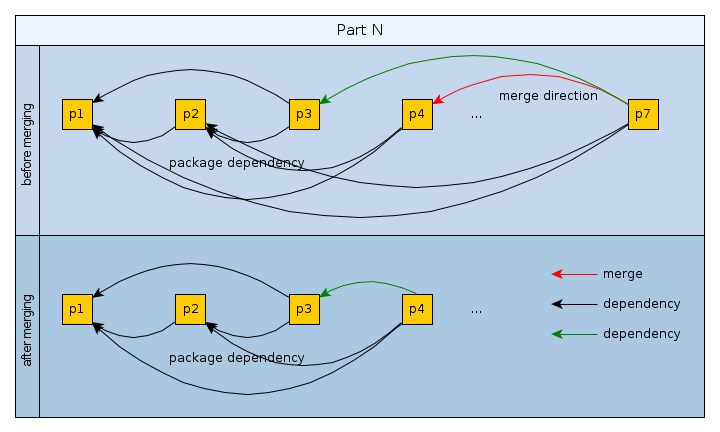
\includegraphics[width=20in]{g_package_merging.png} \\
          \caption{Merging packages and maintaining dependencies}
          \label{fig:corrSubsys}
        \end{center}
      \end{figure}

    % middle bottom

    \begin{columns}[t,totalwidth=\twocolwid]
    \begin{column}{\onecolwid}

      \begin{block}{Target Package Selection}
        The following conditions have to be met for a package to be eligible as a
        merge target.
        \begin{itemize}
          \item $Parts(p_s) \subset Parts(p_t)$ [ this assures the classes of
            $p_s$ remain avaiable wherever they are needed ]
          \item ???
        \end{itemize}
      \end{block}

      \vskip2ex
      \begin{block}{Merging by Load Order}
        The aim of load-order merging is to have just one additional package to
        load with each new part.

        \begin{itemize}
          \item By using the \textit{expected-load-order} configuration key the
            user groups together parts (\textit{load groups}) where the number
            indicates the expected load order.
          \item This allows for more aggressive package merging.
          \item As a corner case, a load group can consist of a single part.
          \item Without this configuration key, or within a single group, no
            load order is assumed.
          \item First, all \textit{unique} packages within the load group are merged.
        \end{itemize}

      \end{block}


    \end{column}
    \begin{column}{\onecolwid}

      % continue previous section
      \begin{block}{ }
        \begin{itemize}
          \item Then, packages \textit{common} among the parts of the load group are
            merged.
          \item Target packages are only used \textbf{once}. This is to avoid
            ``monster packages''.
          \item The \textit{boot} part is always load order-merged by default. It
            has load order number \textit{0} which cannot be assigned to any
            other load group.
          \item Parts which are not in any load group are not actively
            collapsed. (They are still affected by package changes if packages
            they use are merged).
        \end{itemize}

      \end{block}
      \vskip2ex
      \begin{block}{References}
        The following qooxdoo applications use parts, with and without explicit
        load-ordering:

        \small{\begin{thebibliography}{99}
          \bibitem FFeedreader Configuration, (load groups commented out),
            {\scriptsize https://github.com/qooxdoo/qooxdoo/blob/release\_3\_0\_1/application/feedreader/config.json}
          \bibitem WWidgetBrowser Configuration, (no load groups)
            {\scriptsize https://github.com/qooxdoo/qooxdoo/blob/release\_3\_0\_1/application/widgetbrowser/config.json}
          \bibitem 33C MailClient Parts Configuration, (2 load groups)
            {\scriptsize https://svn.1and1.org/svn/ccclient/qooxdoo-client/trunk/conf/parts.json}
        \end{thebibliography}}
      \end{block}

    \end{column}
    \end{columns}
    \end{column}  % 2-column middle

    % column 4

    \begin{column}{\sepwid}\end{column}			% empty spacer column

    \begin{column}{\onecolwid}

      \begin{block}{Merging by Load Order (cont.)}
        Load-order merging \textbf{does not} destroy the ability to load parts
        \textit{in arbitrary order}. But if parts are loaded out of order
        a larger number of unneeded classes will be loaded with the required
        packages.
      \end{block}

      \vskip2ex
      \begin{block}{Questions}
        \begin{itemize}
          \item The condition for a target package is trivially true in the
            sorted list of part packages. Why?
          \item Parts which don't belong to any load group are not processed in
            the load-order phase. Why?
          \item Whithin a load group, why are unique packages processed first,
            then common packages?
          \item Why are merge targets restricted to one use only?
        \end{itemize}


        \vskip2ex
        \begin{figure}
          \begin{center}
            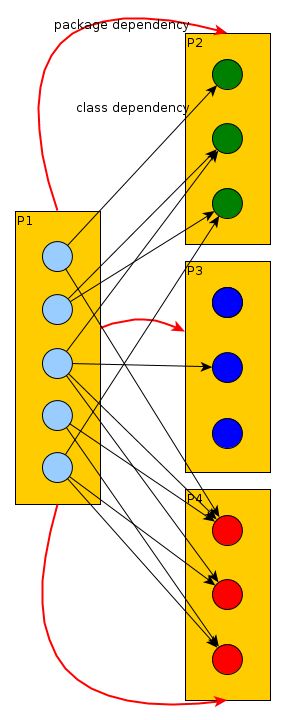
\includegraphics[width=6in]{g_package_deps.png}
            \caption{Class dependencies induce package dependencies}
            \label{fig:corrSubsys}
          \end{center}
        \end{figure}

      \end{block}

    \end{column}

  \end{columns}
\end{frame}
\end{document}
